\section{Översikt av system}
På plattformen kommer tre moduler att installeras:

\begin{itemize}
\item Huvudmodul
\item Styrmodul
\item Sensormodul
\end{itemize}
Huvudmodulen kommer troligvis bestå av en Beagleboard-xM. Sensormodulen och styrmodulen ska förslagsvis bestå av varsin Atmega16.
\subsection{Kommunikation}
Kommunikationen mellan Huvudmodulen, styrmodulen och sensormodulen kommer förslagsvis att ske över UART. Huvudmodulen kommer isåfall ha två stycken USB-RS232 konverterare som kommer kopplas till varsin modul. Kommunikationen från huvudmodulen till PC kommer att ske över Bluetooth. Förslaget är att sätta upp ett PAN (PERSONAL AREA NETWORK) mellan PC:n och huvudmodulen. Detta möjliggör kommunikation över TCP/IP protokollet.
%\newline
%\centerline{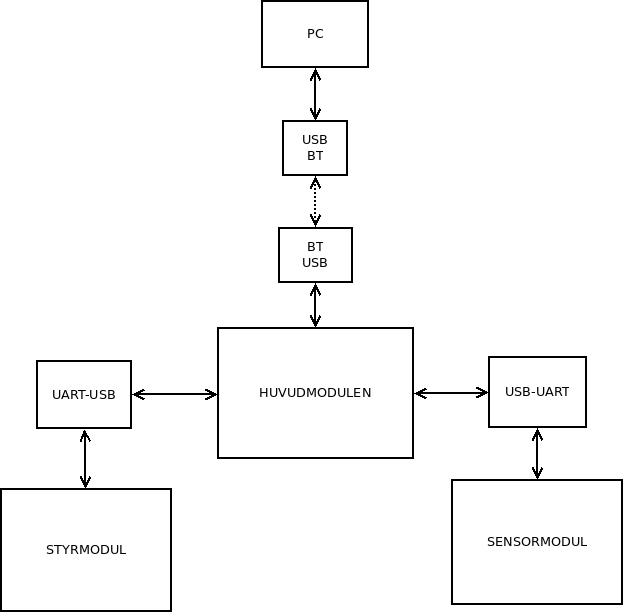
\includegraphics[scale=0.4]{FLOW1PNG}}
%\centerline{Flödesschema över kommunikationen i systemet}
%\newline
%\newline
%\centerline{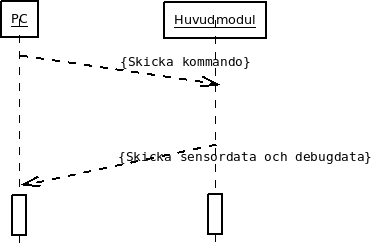
\includegraphics[scale=0.6]{PC-huvud}}
%\centerline{Kommunikation mellan PC och huvudmodulen}
%\newline
%\newline
%\centerline{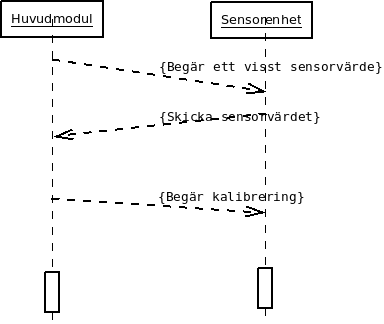
\includegraphics[scale=0.6]{huvud-sensor}}
%\centerline{Kommunikation mellan huvudmodulen och sensormodulen}
%\newline
%\newline
%\centerline{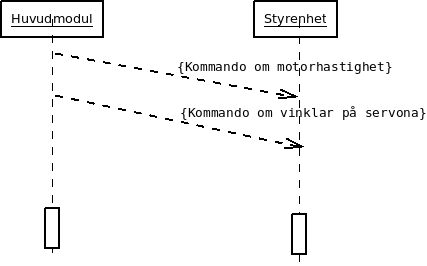
\includegraphics[scale=0.6]{huvud-styr}}
%\centerline{Kommunikation mellan huvudmodulen och styrmodulen}

\begin{figure}[h]
\center
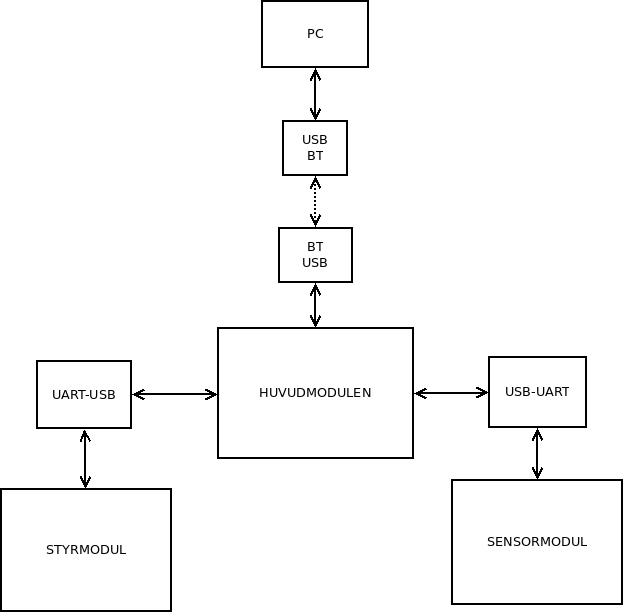
\includegraphics[scale=0.3]{FLOW1PNG}
\caption{Flödesschema över kommunikation i systemet.}
\end{figure}

\begin{figure}[h]
\center
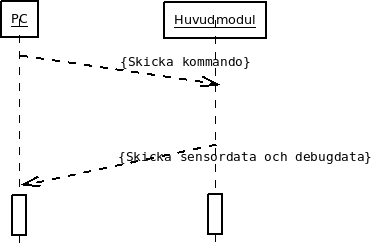
\includegraphics[scale=0.6]{PC-huvud}
\caption{Kommunikation mellan PC och huvudmodulen.}
\end{figure}

\begin{figure}[h]
\center
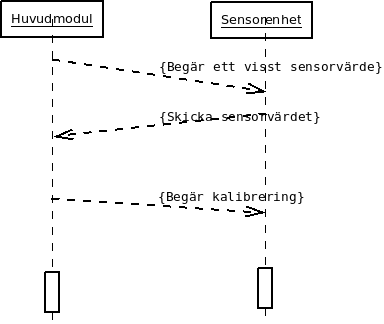
\includegraphics[scale=0.6]{huvud-sensor}
\caption{Kommunikation mellan huvudmodulen och sensormodulen.}
\end{figure}

\begin{figure}[h]
\center
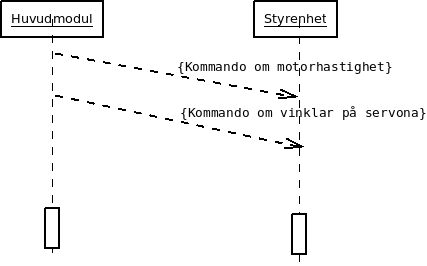
\includegraphics[scale=0.6]{huvud-styr}
\caption{Kommunikation mellan huvudmodulen och styrmodulen.}
\end{figure}

\subsection{Uppgraderbarhet}
Tydliga kommunikationsprotokoll ska existera eftersom det blir enklare att byta ut en modul. Kommunikationen mellan huvudmodulen och övriga moduler sker förslagsvis över UART. Eftersom detta sker med hjälp av USB-UART donglar så finns det möjlighet att lägga till fler moduler i framtiden eftersom Beagleboarden har fyra USB-portar och tre kommer användas i systemet. Behövs fler i framtiden så kan en USB-hubb användas.
\newline
\newline
Kommunikationen mellan huvudmodulen och PC:n kommer förslagsvis att ske över bluetooth och isåfall kommer den användas för att sätta upp ett PAN. Över denna sätts en TCP/IP anslutning upp och data skickas över en Python-socket vilket leder till att bluetooth kan bytas ut mot WIFI eller en ethernetkabel.
